\documentclass[letterpaper,12pt,fleqn]{article}
\usepackage{matharticle}
\pagestyle{empty}
\begin{document}
\section*{Mappings}

\begin{example}[Translation]
  $w=f(z)=z+1$

  \begin{minipage}{2in}
    \begin{tikzpicture}
      \draw [->] (0,0) -- (3,0) node [right] {$x$};
      \draw [->] (0,0) -- (0,3) node [above] {$y$};
      \node [below] at (0,0) {$0$};
      \draw (1,0) node [below] {$1$} -- (1,1) node [above] {$1+i$} --
      (0,1) node [left] {$i$};
    \end{tikzpicture}
  \end{minipage}
  \begin{minipage}{1.5in}
    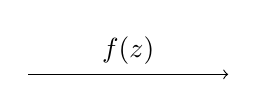
\begin{tikzpicture}
      \draw [->] (0,0) -- node [above] {$f(z)$} (1in,0);
    \end{tikzpicture}
  \end{minipage}
  \begin{minipage}{2in}
    \begin{tikzpicture}
      \draw [->] (0,0) -- (3,0) node [right] {$u$};
      \draw [->] (0,0) -- (0,3) node [above] {$v$};
      \draw (1,0) node [below] {$1$} -- (1,1) node [above] {$1+i$} --
      (2,1) node [above] {$2+i$} -- (2,0) node [below] {$2$};
    \end{tikzpicture}
  \end{minipage}
\end{example}

\begin{example}[Scaling]
  $w=f(z)=2z$

  \begin{minipage}{2in}
    \begin{tikzpicture}
      \draw [->] (0,0) -- (3,0) node [right] {$x$};
      \draw [->] (0,0) -- (0,3) node [above] {$y$};
      \node [below] at (0,0) {$0$};
      \draw (1,0) node [below] {$1$} -- (1,1) node [above] {$1+i$} --
      (0,1) node [left] {$i$};
    \end{tikzpicture}
  \end{minipage}
  \begin{minipage}{1.5in}
    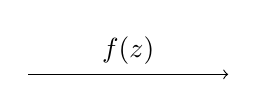
\begin{tikzpicture}
      \draw [->] (0,0) -- node [above] {$f(z)$} (1in,0);
    \end{tikzpicture}
  \end{minipage}
  \begin{minipage}{2in}
    \begin{tikzpicture}
      \draw [->] (0,0) -- (3,0) node [right] {$u$};
      \draw [->] (0,0) -- (0,3) node [above] {$v$};
      \node [below] at (0,0) {$0$};
      \draw (2,0) node [below] {$2$} -- (2,2) node [above] {$2+2i$} --
      (0,2) node [left] {$2i$};
    \end{tikzpicture}
  \end{minipage}
\end{example}

\begin{example}[Rotation]
  $w=f(z)=(1+i)z=(\sqrt{2}e^{i\frac{\pi}{4}})z$

  \begin{minipage}{2.5in}
    \begin{tikzpicture}
      \draw [<->] (-3,0) -- (3,0) node [right] {$x$};
      \draw [->] (0,0) -- (0,3) node [above] {$y$};
      \node [below] at (0,0) {$0$};
      \draw (1,0) node [below] {$1$} -- (1,1) node [above] {$1+i$} --
      (0,1) node [left] {$i$};
    \end{tikzpicture}
  \end{minipage}
  \begin{minipage}{0.75in}
    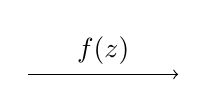
\begin{tikzpicture}
      \draw [->] (0,0) -- node [above] {$f(z)$} (0.75in,0);
    \end{tikzpicture}
  \end{minipage}
  \begin{minipage}{3in}
    \begin{tikzpicture}
      \draw [<->] (-3,0) -- (3,0) node [right] {$x$};
      \draw [->] (0,0) -- (0,3) node [above] {$y$};
      \draw (0,0) [below] node {$0$} --
      (1,1) node [right] {$1+i$} --
      (0,2) node [above] {$2i$} --
      (-1,1) node [left] {$-1+i$} -- (0,0);
    \end{tikzpicture}
  \end{minipage}
\end{example}
\newpage
\begin{example}
  $w=f(z)=z^2=(x^2-y^2)+i2xy$

  \begin{minipage}{3.5in}
    \begin{tikzpicture}
      \draw [<->] (-3,0) -- (3,0) node [right] {$x$};
      \draw [->] (0,-3) -- (0,3) node [above] {$y$};
      \draw [->] (3.5,1) -- node [above] {$f(z)$} (5.5,1);
      \draw (0,0) -- node [left] {$y=x$} (1,1) -- (1,-1) --
      node [left] {$y=-x$} (0,0);
      \node [below right] at (1,0) {$1$};
    \end{tikzpicture}
  \end{minipage}
  \begin{minipage}{3in}
    \begin{tikzpicture}
      \draw [<->] (-3,0) -- (3,0) node [right] {$x$};
      \draw [->] (0,-3) -- (0,3) node [above] {$y$};
      \node [left] at (0,2) {$2$};
      \node [left] at (0,-2) {$-2$};
      \node [below right] at (1,0) {$1$};
      \draw [domain=0:1] plot ({\x},{sqrt(4-4*\x)});
      \draw [domain=0:1] plot ({\x},{-sqrt(4-4*\x)});
    \end{tikzpicture}
  \end{minipage}

  Along $y=x$ from $x=0$ to $1$: \\
  $u=0$ and $v=2x^2$
  
  Along $y=-x$ from $x=0$ to $1$: \\
  $u=0$ and $v=-2x^2$

  Along $x=1$: \\
  $u=1-y^2$ and $v=2y$ \\
  $u=1-(\frac{v}{2})^2$ \\
  $4u=4-v^2$ \\
  $v^2=-4(u-1)$
\end{example}

\begin{example}
  $w=f(z)=\frac{1}{z}=\frac{x}{x^2+y^2}-i\frac{y}{x^2+y^2}$
  
  $u=\frac{x}{x^2+y^2}$ and $v=-\frac{y}{x^2+y^2}$ \\
  But since $z=\frac{1}{w}$: \\
  $x=\frac{u}{u^2+v^2}$ and $y=-\frac{v}{u^2+v^2}$ \\

  $\abs{w}=\frac{1}{\abs{z}}$ \\
  So the circle $\abs{z}=r$ maps to the circle $\abs{w}=\frac{1}{r}$

  $\abs{w}^2=\frac{1}{\abs{z}^2}$ \\
  $u^2+v^2=\frac{1}{x^2+y^2}$ \\
  $x^2+y^2=\frac{1}{u^2+v^2}$
\newpage
  Consider the circle $a(x^2+y^2)+bx+cy+d=0$ and apply the mapping:
  \[a(\frac{1}{u^2+v^2})+b(\frac{u}{u^2+v^2})+c(-\frac{v}{u^2+v^2})+d=0\]
  \[d(u^2+v^2)+bu-cv+a=0\]
  So as long as $a,d\ne0$, a circle is mapped to a circle.
\end{example}

\end{document}
